%!TEX program = pdflatex
% ============================================================
%  TEMPLATE CV deux colonnes « Informatique x Recherche » — 1 page
%  Alexis MIALON — inspiré de l'ancien CV (barre latérale + frise)
%  Compilation : pdflatex cv_alexis_mialon_2col.tex  (x2, pour la frise)
%  Photo : placer photo.jpg à côté du .tex (sinon la photo est omise)
% ============================================================
\documentclass[10pt,a4paper]{article}

\usepackage[utf8]{inputenc}
\usepackage[T1]{fontenc}
\usepackage[scaled=0.92]{helvet}
\renewcommand{\familydefault}{\sfdefault}
\usepackage[a4paper,margin=0pt,nohead,nofoot]{geometry}
\usepackage{xcolor}
\usepackage{graphicx}
\usepackage{eso-pic}
\usepackage{tikz}
\usetikzlibrary{calc}
\usepackage{enumitem}
\usepackage[hidelinks,pdftitle={CV - Alexis Mialon},pdfauthor={Alexis Mialon}]{hyperref}

% ---------- Couleurs (modifier ici pour changer le thème) ----------
\definecolor{accent}{HTML}{2EA3E0}   % bleu des titres
\definecolor{side}{HTML}{232323}     % fond de la barre latérale
\definecolor{sidetext}{HTML}{D6D6D6} % texte secondaire de la barre
\definecolor{ink}{HTML}{222222}      % titres sombres
\definecolor{body}{HTML}{4A4A4A}     % texte courant
\definecolor{muted}{HTML}{777777}

% ---------- Dimensions ----------
\newcommand{\sidew}{6.1cm}      % largeur de la barre latérale
\newcommand{\sidetextw}{4.7cm}  % largeur utile du texte de la barre
\newcommand{\maintextw}{12.5cm} % largeur de la colonne principale

\AddToShipoutPictureBG*{\AtPageLowerLeft{\color{side}\rule{\sidew}{\paperheight}}}

\pagestyle{empty}
\setlength{\parindent}{0pt}
\setlength{\parskip}{0pt}
\setlist[itemize]{leftmargin=0.9em,itemsep=0pt,topsep=1pt,parsep=0pt,label={\textcolor{muted}{\textbullet}}}
\raggedright

% ---------- Barre latérale ----------
\newcommand{\sidehead}[1]{\vspace{9pt}{\color{white}\bfseries\large #1}\par\vspace{3pt}}
\newcommand{\sideitem}[2]{{\color{white}\bfseries\small #1}\\[-1pt]{\color{sidetext}\footnotesize #2}\par\vspace{3pt}}
\newcommand{\sideline}[1]{{\color{white}\footnotesize #1}\par\vspace{2pt}}

% ---------- Frise (colonne principale) ----------
\newsavebox{\eb}
% \entryfull{rallonge}{Titre}{Date}{Organisation}{Lieu}{Description}
% Chaque entrée dessine son point et son segment de frise (pas de 2e compilation).
\newcommand{\entryfull}[6]{%
  \vspace{4.5pt}\noindent%
  \sbox{\eb}{\begin{minipage}[t]{\maintextw}\raggedright
    {\color{ink}\bfseries\normalsize #2}\par
    {\color{muted}\small #3}\ \ {\color{accent}\small #4}\ \ {\color{muted}\small #5}\par\vspace{1.5pt}
    #6
  \end{minipage}}%
  \tikz[overlay]{%
    \fill[ink] (-0.5cm,-0.11cm) circle (2.7pt);
    \draw[ink,line width=0.9pt] (-0.5cm,-0.11cm) -- (-0.5cm,{-\the\dimexpr\dp\eb+#1+0.11cm\relax});}%
  \usebox{\eb}\par}
% \entry : relié à l'entrée suivante ; \entrylast : dernière entrée d'une section
\newcommand{\entry}[5]{\entryfull{8pt}{#1}{#2}{#3}{#4}{#5}}
\newcommand{\entrylast}[5]{\entryfull{-7pt}{#1}{#2}{#3}{#4}{#5}}

\newcommand{\maintitle}[1]{{\color{accent}\bfseries\large #1}\par\vspace{3pt}}
\newcommand{\desc}[1]{{\color{body}\small #1}\par}
\newcommand{\IT}[1]{\textcolor{ink}{\bfseries #1}}

\begin{document}
\noindent\hspace*{0.65cm}%
\begin{minipage}[t][29.2cm][t]{\sidetextw}\raggedright
  \vspace{0.75cm}
  \IfFileExists{photo.jpg}{\noindent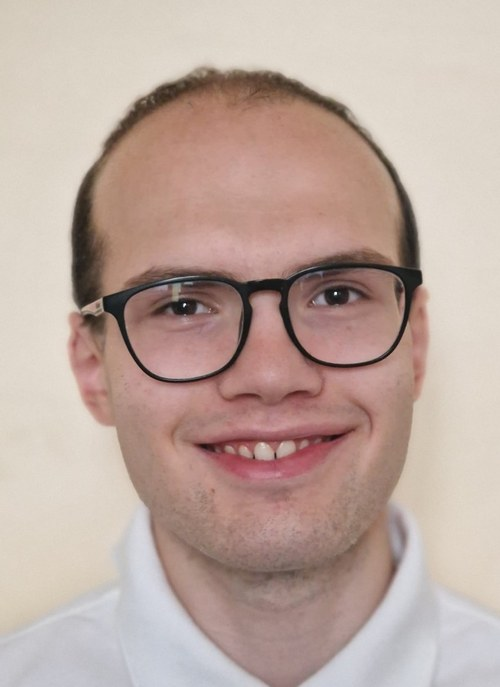
\includegraphics[width=\sidetextw]{photo.jpg}\par\vspace{6pt}}{}
  \sideline{\textcolor{accent}{\textbullet}\ alexis.mialon69@gmail.com}
  \sideline{\textcolor{accent}{\textbullet}\ Lyon}
  \sideline{\textcolor{accent}{\textbullet}\ 06\,76\,15\,68\,88}

  \sidehead{Réseaux}
  \sideline{\href{https://www.linkedin.com/in/alexis-mialon-79117b329/}{\textcolor{white}{linkedin.com/in/}}\\\href{https://www.linkedin.com/in/alexis-mialon-79117b329/}{\textcolor{white}{alexis-mialon-79117b329}}}
  \sideline{\href{https://github.com/Vorpalin}{\textcolor{white}{github.com/Vorpalin}}}
  \sideline{\href{https://vorpalin.github.io/}{\textcolor{white}{vorpalin.github.io}}}

  \sidehead{Langues}
  \sideitem{Français}{Langue maternelle}
  \sideitem{Anglais}{Niveau C1 · TOEIC 960/990}
  \sideitem{Italien}{Notions}

  \sidehead{Compétences}
  \sideitem{Langages}{C, C++ (C++20), Python, Java, C\#, JavaScript / TypeScript, SQL}
  \sideitem{IA \& recherche}{IA agentique, cryptanalyse différentielle, programmation dynamique, calcul parallèle}
  \sideitem{Web \& WASM}{React, Vite, WebAssembly (Emscripten), HTML/CSS, API REST}
  \sideitem{Outils}{Git (GitHub, GitLab), CI/CD, Docker, CMake, Linux (NixOS), JUnit}
  \sideitem{Bases de données}{PostgreSQL, MySQL}

  \sidehead{Distinctions}
  \sideitem{Top Scorer 2026}{Challenge du Meilleur étudiant en informatique de France}
  \sideitem{Open source}{2 PR fusionnées dans langchain-aws}

  \sidehead{Centres d'intérêt}
  \sideitem{Tennis de table}{Départemental 1 en équipe, pré-régional en individuel}
  \sideitem{Cinéma}{}
\end{minipage}%
\hspace{1.75cm}%
\begin{minipage}[t][29.2cm][t]{\maintextw}\raggedright
  \vspace{0.75cm}
  {\color{ink}\bfseries\Large Alexis MIALON}\par\vspace{2pt}
  {\color{accent}\bfseries\Large Informatique \& Recherche}\par\vspace{3pt}
  {\color{body}\small Élève-ingénieur à l'EPITA (diplôme prévu en 2028), stagiaire IA chez Opensee et étudiant-chercheur en cryptanalyse différentielle. Je cherche à travailler là où l'ingénierie logicielle, l'IA et la recherche se rencontrent.}\par

  \vspace{7pt}\maintitle{Expériences}
  \entry{Stagiaire IA}{Sept. 2026 -- présent}{Opensee}{Puteaux}{%
    \desc{Contribution au développement d'\IT{Agensee}, solution d'IA agentique dédiée à l'analyse de données financières, au sein de l'équipe IA.}}
  \entry{Étudiant-chercheur, équipe Sécurité \& Systèmes}{Depuis fév. 2026}{LRE (EPITA)}{Lyon}{%
    \begin{itemize}\small\color{body}
      \item Optimisation de la minimisation des \IT{S-boxes actives} dans l'outil de cryptanalyse différentielle \IT{TAGADA} : algorithmes de programmation dynamique \IT{multithreadés en C++}.
      \item Automatisation de la récupération des tours de chiffrement (parsing JSON), benchmarks conteneurisés (Docker), synthèse des avancées à l'équipe.
    \end{itemize}}
  \entry{Assistant pédagogique en programmation}{2025 -- 2026}{EPITA, SupBiotech}{Lyon}{%
    \desc{Accompagnement quotidien d'étudiants de première année en \IT{C} et \IT{Python}, Git et Linux ; relecture des sujets et tests de TP, correction (Criterion, GitLab).}}
  \entrylast{Bénévole}{2016 -- 2023}{Ensemble scolaire Charles de Foucauld}{Lyon}{%
    \desc{Animation d'activités (escape game), tenue de caisse, référent de stand avec une équipe d'une vingtaine de personnes.}}

  \vspace{6pt}\maintitle{Projets \& open source}
  \entry{Contributions à langchain-aws (LangChain)}{Oct. 2026}{2 PR fusionnées}{\href{https://github.com/langchain-ai/langchain-aws/pull/1389}{\#1389}, \href{https://github.com/langchain-ai/langchain-aws/pull/1415}{\#1415}}{%
    \desc{Ajout des niveaux d'effort de raisonnement (\texttt{reasoning\_effort\_levels}) aux profils de modèles Amazon Bedrock ; lint et tests validés.}}
  \entry{Emulators Collection}{Projet personnel}{C++20, WebAssembly, React}{\href{https://github.com/Vorpalin/emulators-collection}{GitHub}}{%
    \desc{Émulateurs \IT{CHIP-8, Super-CHIP, Atari 2600 et Game Boy} : cœurs C++20 compilés en \IT{WebAssembly}, frontend React/TypeScript ; CI GitHub Actions, analyse de sécurité, releases automatiques.}}
  \entry{PING, IDE en ligne pour débutants}{Depuis mars 2026}{EPITA}{Équipe agile de 5}{%
    \desc{Conception produit (état de l'art, interviews, maquettes), interface React, backend Java testé par pipeline CI/CD GitLab, documentation Javadoc.}}
  \entrylast{42sh, shell POSIX en C}{Janv. 2026}{EPITA}{Équipe agile de 4}{%
    \desc{Lexer et parser, architecture fondée sur les patrons \IT{visiteur} et \IT{composite}, revue des merge requests GitLab. Autre projet : Yakamon, API REST Java en couches avec JUnit.}}

  \vspace{6pt}\maintitle{Diplômes et formations}
  \entry{Diplôme d'ingénieur en informatique}{Depuis sept. 2023}{EPITA}{Lyon}{}
  \entry{Semestre à l'étranger, Computer Science}{Jan. -- mai 2025}{Centria University of Applied Sciences}{Kokkola, Finlande}{}
  \entrylast{Baccalauréat général}{Juil. 2023}{Lycée Charles de Foucauld}{Lyon}{}
\end{minipage}
\end{document}
